\documentclass[submit]{harvardml}

\course{STAT184-F22}
\assignment{Assignment \#0}
\duedate{11:59pm EST, Sept. 7, 2022}
\name{Rodney Lafuente Mercado}

\usepackage{subfig}
\usepackage{framed}
\usepackage{fullpage}
\usepackage{amsmath}
\usepackage{amssymb}
\usepackage{color}
\usepackage{todonotes}
\usepackage{listings}
\usepackage{common}
\usepackage{bm}
\usepackage{enumitem}
\usepackage{pythonhighlight}
\usepackage{soul}
\usepackage{mathtools}

\usepackage[mmddyyyy,hhmmss]{datetime}


\begin{document}

\renewcommand{\labelenumii}{\arabic{enumi}.\arabic{enumii}}
\renewcommand{\labelenumiii}{(\alph{enumiii})}

\begin{enumerate}
  \item Policies
  \begin{enumerate}
    \item
    List of Collaborators:
    I did not collaborate with anyone on this assignment
    
    \item
    List of Acknowledgements: None
    
    \item
    Certification of Reading of Instructions: 
    I have read these policies
  \end{enumerate}

  \item Website
  \begin{enumerate}
    \item 
    I have read the course policies on the website.
  \end{enumerate}

  \item Bayes
  \begin{enumerate}
    \item
    Let $D$ be the event that I test positive and let $P$ be the event that I test negative. That 
    means that I have $P(D) = 0.0001$ and $P(P|D) = 0.99$.

    By applying Bayes Rule, we get the following:

    $$P(D|P) = \frac{P(P|D)P(D)}{P(P)} = \frac{P(P|D)P(D)}{P(P|D)P(D) + P(P|D^C)P(D^C)}$$
    $$= \frac{0.99 \cdot 0.0001}{0.99\cdot 0.0001 + 0.001 \cdot 0.9999} \approx 0.0098 
    = \boxed{0.98\%}$$
  \end{enumerate}


  \item Probability
  \begin{enumerate}
    \item
    In the discrete case, we have
    $$P(Z=z) = \sum_{z\in\mathbb{R}} P(X=x,Y=z-x)$$
    this expresses the probability that, given a value for $x$, $y$ is exactly its difference to 
    $z$. Since $X$ and $Y$ are independent, we have
    $$P(Z=z) = \sum_{z\in\mathbb{R}} P(X=x)P(Y=z-x)$$
    In the continuous case, this translates to
    $$h(z) = \int_{-\infty}^{\infty} f(x)g(x-z)dx$$
    since we are ``summing" over all possibilities for $x$ times their infinitesimal probabilities
    of occurring.


    \item
    \begin{enumerate}
      \item 
      We have 
      
      $$h(z) = \int_{-\infty}^{\infty} f(x)g(x-z)dx$$

      $f(x) = 0$ for $x \notin [0,1]$ and 1 otherwise:

      $$h(z) = \int_{0}^{1} g(x-z)dx$$

      $g(x-z) = 1$ if $0 \leq x-z \leq 1$ and 0 otherwise. We have two cases for which 
      $0 \leq x-z \leq 1$: 

      Case 1: $0\leq z\leq 1$: In this case, $h(z) = z$ as the integral will be non-zero only 
      for $0\leq x\leq z$.

      Case 2: $1\leq z\leq 2$: In this case, $h(z) = 2-z$. As the integral will be non-zero only for
      $z-1\leq x\leq 1$.

      Hence, we have

      $$
      \boxed{
      h(z) =
      \begin{dcases} 
        z & 0\leq z\leq 1 \\
        2-z & 1\leq z\leq 2\\
        0 & \textnormal{otherwise}
      \end{dcases}
      }
      $$

      \item
      We have
      $$P(X\leq 1/2 | X + Y \geq 5/4) = P(X\leq 1/2 | Z\geq 5/4)
        = \frac{P(X\leq 1/2, Z \geq 5/4)}{P(Z \geq 5/4)}$$
      
      We also have that the joint PDF of $X,Z$ is 
      $$f_{X,Z}(x,z)=1_{\{0\leq x\leq 1, x\leq z\leq x+1\}}$$

      Therefore, we have, in the numerator,
      $$P(X\leq 1/2 | Z\geq 5/4)$$
      $$=\int_0^{1/2} \int_{5/4}^2 f_{X,Z} (x,z) dz dx$$
      $$=\int_0^{1/2} \int_{5/4}^2 1_{\{0\leq x\leq 1, x\leq z\leq x+1\}} dz dx$$
      $$=\int_0^{1/2} \int_{5/4}^2 1_{\{x\leq z\leq x+1\}} dz dx$$
      $$=\int_{1/4}^{1/2} \int_{5/4}^{3/2} 1_{\{x\leq z\leq x+1\}} dz dx$$
      $$=\int_{1/4}^{1/2} \int_{5/4}^{x+1} 1\, dz dx$$
      $$=\int_{1/4}^{1/2} x + 1 - 5/4\, dx$$
      $$=\int_{1/4}^{1/2} x + 1 - 5/4\, dx$$
      $$=\int_{1/4}^{1/2} x - 1/4\, dx$$
      $$=P(X\leq 1/2 | Z\geq 5/4)=1/32$$

      In the denominator we have
      $$P(Z \geq 5/4)$$
      $$=\int_{5/4}^2 h(z) dz$$
      $$=\int_{5/4}^2 2-z dz$$
      $$=9/32$$

      Putting this together we have
      $$P(X\leq 1/2 | X + Y \geq 5/4) = P(X\leq 1/2 | Z\geq 5/4)
      = \frac{P(X\leq 1/2, Z \geq 5/4)}{P(Z \geq 5/4)}$$
      $$=\frac{1/32}{9/32}$$
      $$\boxed{P(X\leq 1/2 | X + Y \geq 5/4)=1/9}$$
    \end{enumerate}

    \item
    Let $G$ be the CDF of $Y$. Then we have 
    $$G(y) = P(Y\leq y) = P(aX+b \leq y) = P(X\leq \frac{y-b}{a}) = F(\frac{y-b}{a})$$

    Through differentiation we get the PDF of $Y$:
    $$g(y) = \frac{1}{a} f(\frac{y-b}{a})$$
    $$=\frac{1}{a}\frac{1}{\sigma\sqrt{2\pi}} e^{-1/2 \left( \frac{\frac{y-b}{a} -\mu}{\sigma} \right) ^2}$$
    $$=\frac{1}{(a\sigma)\sqrt{2\pi}} e^{-1/2 \left( \frac{y-(a\mu+b)}{(a\sigma)} \right) ^2}$$

    Which is the PDF of a random variable with distribution $\mathcal{N}(a\mu+b, a^2\sigma^2)$.

    In order for $Y\sim \mathcal{N}(0,1)$, therefore, we need $a\mu+b=0$ and $a^2\sigma^2=1$. This 
    is accomplished with 
    $$\boxed{a=1/\sigma} \textnormal{ and }\boxed{b=-\mu/b}$$
  
    \item
    \begin{enumerate}
      \item 
      We have 
      $$E[XY] = E[E[XY|X=x]]$$
      $$=E[E[xY|X=x]]$$
      $$=\int_{-\infty}^\infty E[xY|X=x] f_X (x)$$
      $$=\int_{-\infty}^\infty x E[Y|X=x] f_X (x)$$
      $$=\int_{-\infty}^\infty x^2 f_X (x)$$
      $$=E[X^2]$$

      We also have 
      $$E[Y]=E[E[Y|x]]$$
      $$=\int_{-\infty}^\infty E[Y|X=x] f_X(x) dx$$
      $$=\int_{-\infty}^\infty x f_X(x) dx$$
      $$=E[x]$$

      Putting this together we have
      $$\mathrm{Cov}(X,Y) = E[XY] - E[X]E[Y]$$
      $$= E[X^2] - E[X]^2 = E[(X-E[X])^2]$$

      \item
      We have 
      $$\mathrm{Cov}(X,Y) = E[XY] - E[X]E[Y]$$
      If $X,Y$ are independent then we have
      $$\mathrm{Cov}(X,Y) = E[XY] - E[X]E[Y] = E[X]E[Y] - E[X]E[Y] = 0$$
    \end{enumerate}

    \item
    \begin{enumerate}
      \item 
      We have 
      $$E[\hat{F}_n(x)] = E\left[\frac{1}{n} \sum_{i=1}^n 1_{\{X_i\leq x\}}\right]$$
      $$= \frac{1}{n} \sum_{i=1}^n E\left[ 1_{\{X_i\leq x\}}\right]$$
      $$= \frac{1}{n} \sum_{i=1}^n F(x)$$
      $$= F(x)$$

      \item
      We have
      $$\mathrm{Var}(\hat{F}_1(x)) = E[\hat{F}_1(x)^2] - E[\hat{F}_1(x)]^2$$
      $$= E\left[\left(\frac{1}{n} \sum_{i=1}^1 1_{\{X_i\leq x\}}\right)^2\right] - F(x)^2$$
      $$= E\left[1_{\{X_i\leq x\}}\right] - F(x)^2$$
      $$= F(x) - F(x)^2$$
      $$= F(x)(1-F(x))$$

      \item
      We have
      $$\mathrm{Var}(\hat{F}_n(x)) = E[\hat{F}_n(x)^2] - E[\hat{F}_n(x)]^2$$
      $$= E\left[\left(\frac{1}{n} \sum_{i=1}^n 1_{\{X_i\leq x\}}\right)^2\right] - F(x)^2$$
      $$= \frac{1}{n^2} E\left[\sum_{i=1}^n \sum_{k=1}^n 1_{\{X_i\leq x\}} 1_{\{X_k\leq x\}} \right] - F(x)^2$$
      $$= \frac{1}{n^2} E\left[\sum_{i=1}^n \left( 1_{\{X_i\leq x\}} 1_{\{X_i\leq x\}} + \sum_{k\neq i}^n 1_{\{X_i\leq x\}} 1_{\{X_k\leq x\}} \right) \right] - F(x)^2$$
      $$= \frac{1}{n^2} \sum_{i=1}^n \left( F(x) + \sum_{i\neq k}^n F(x)^2 \right) - F(x)^2$$
      $$= \frac{1}{n} F(x) + \frac{1}{n^2} n (n-1) F(x)^2 - F(x)^2$$
      $$= \frac{1}{n} F(x)(1-F(x))$$

      \item
      We have 
      $$\mathrm{Var}(\hat{F}_n(x))  = \frac{1}{n} F(x)(1-F(x)) $$
      Since $0\leq F(x)\leq 1$ we have $F(x)(1-F(x)) \leq 1/4$ and therefore
      $$\mathrm{Var}(\hat{F}_n(x))  = \frac{1}{n} F(x)(1-F(x))$$
      $$ \leq \frac{1}{n}\cdot\frac{1}{4} = \frac{1}{4n} $$
    \end{enumerate}
  \end{enumerate}

\item Geometry and Linear Algebra
\begin{enumerate}
  \item
  \begin{enumerate}
    \item 
    The drawing is the following
    \begin{figure}[h]
    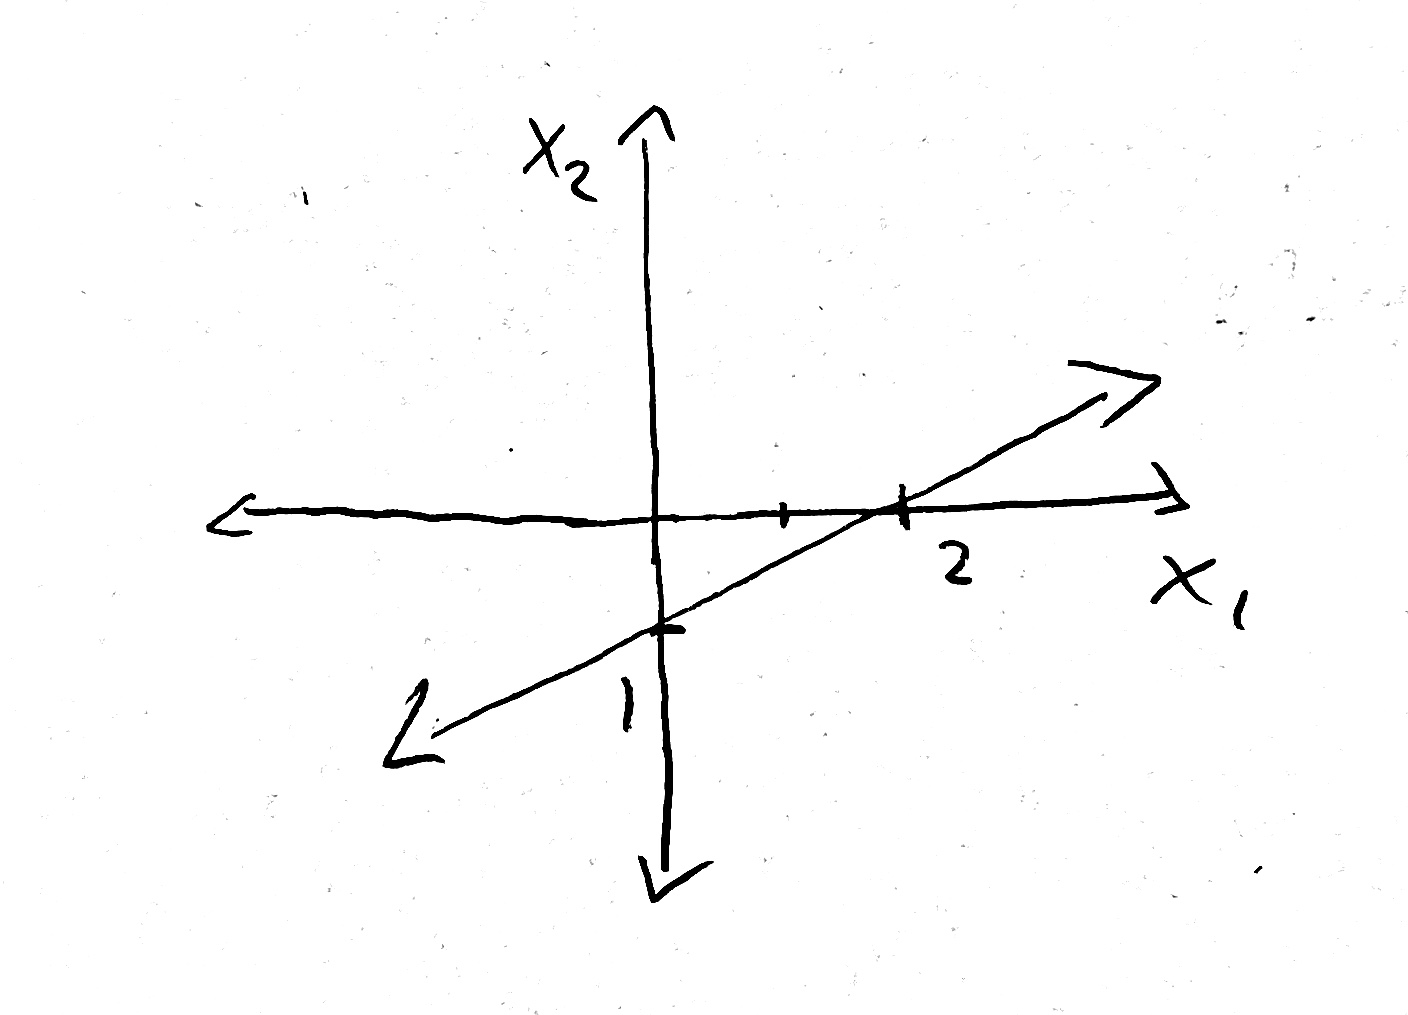
\includegraphics[width=8cm]{ps0_5_1_a}
    \centering
    \end{figure}

    \item 
    The drawing is the following
    \newpage
    \begin{figure}[h]
    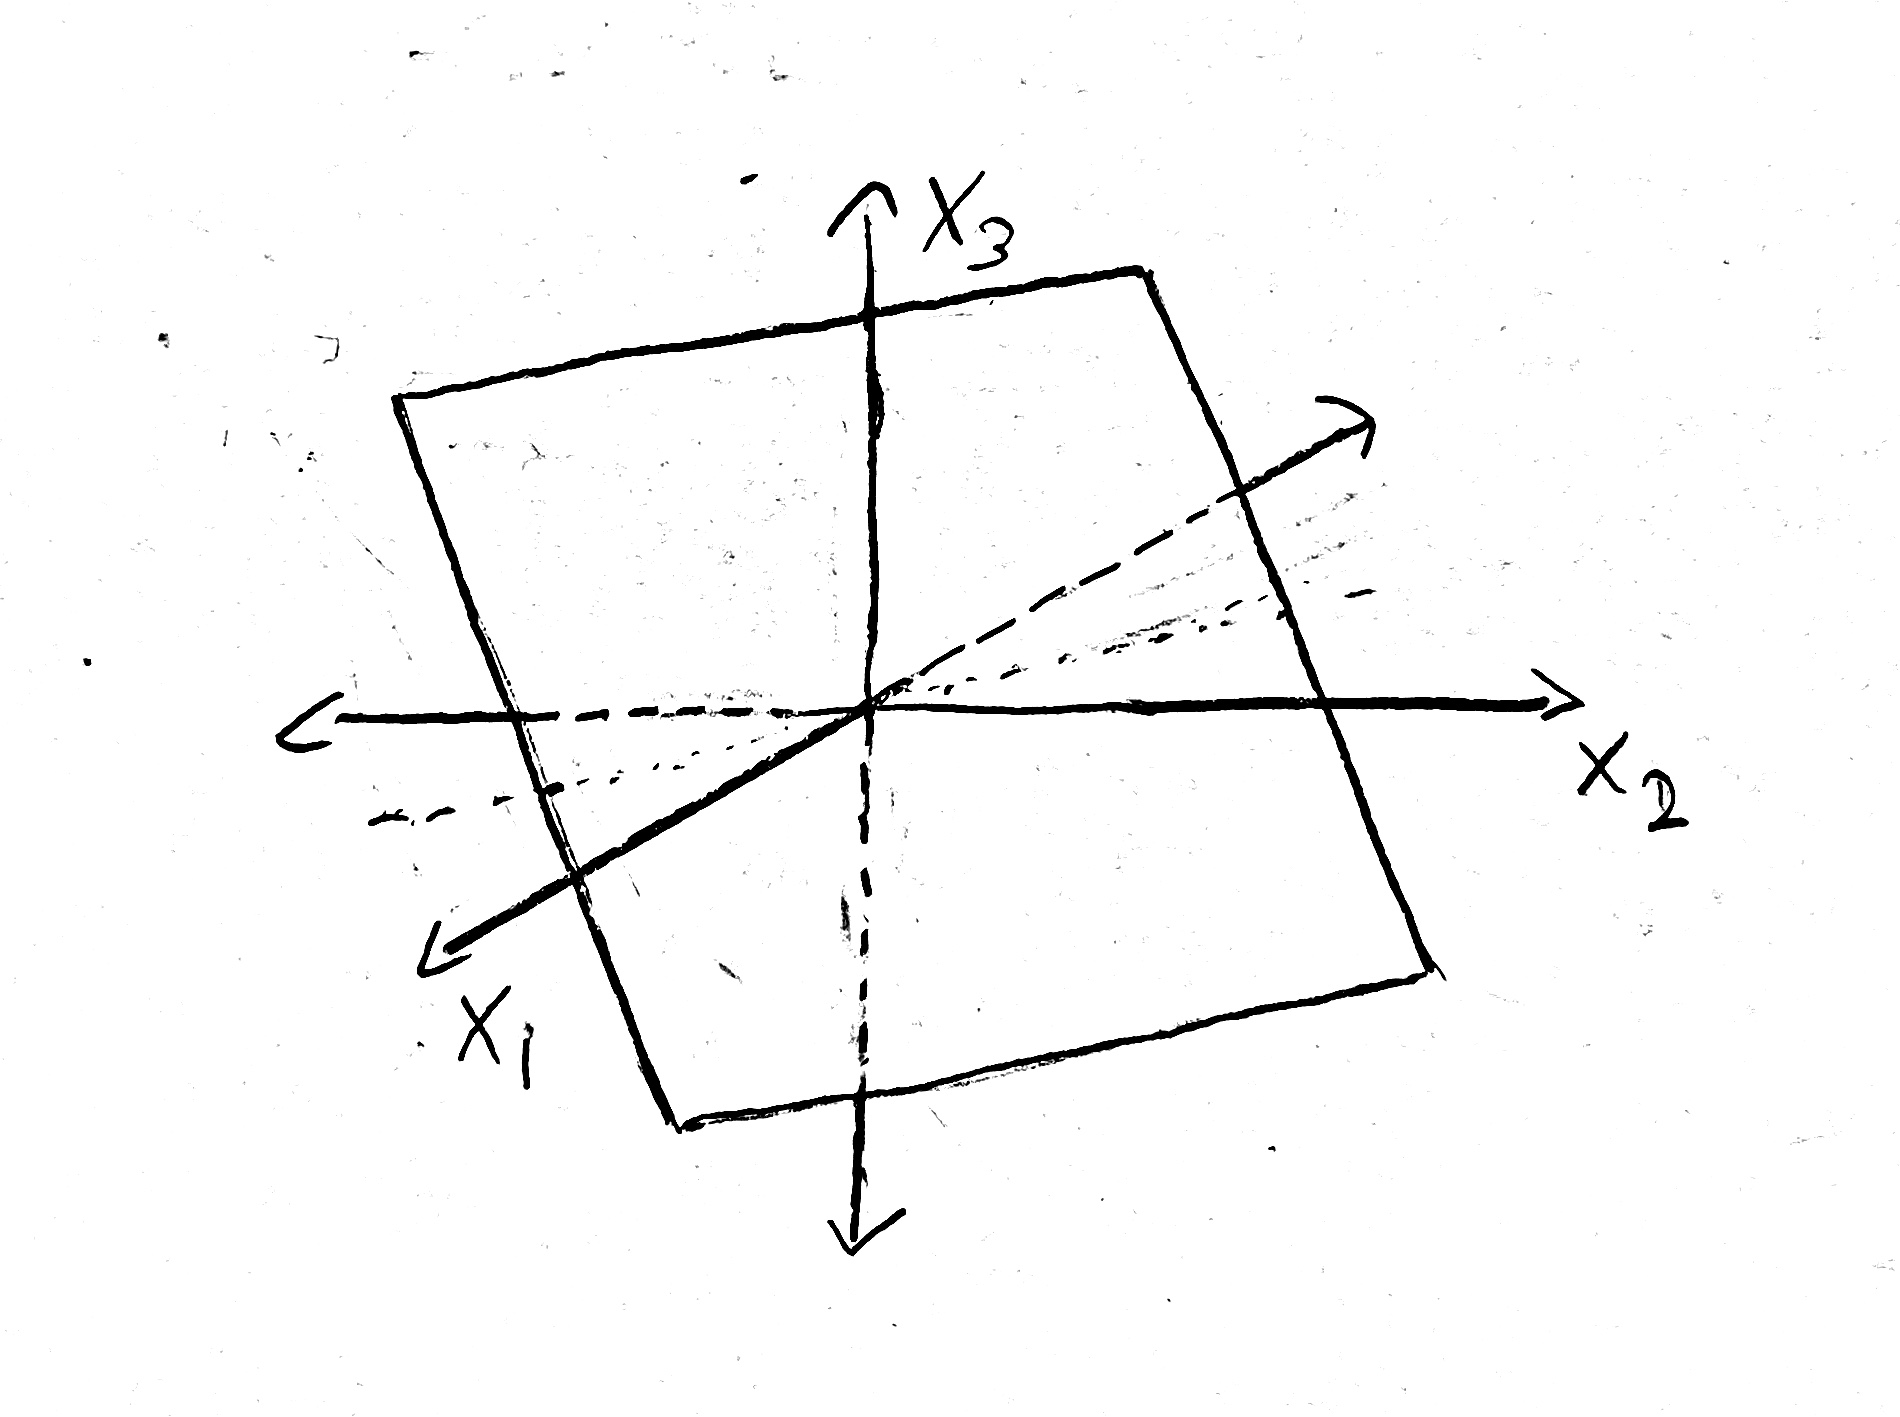
\includegraphics[width=8cm]{ps0_5_1_b}
    \centering
    \end{figure}

    \item
    The problem can be solved using Lagrange Multipliers. The Lagrangian function is
    $$L(x, \lambda) = ||x_0 - x||^2 - \lambda(w^\top x + b)$$

    and the corresponding partial derivatives are
    $$(1)\quad\frac{\partial}{\partial x} L(x, \lambda) = 2(x_0 - x) - \lambda w$$
    $$(2)\quad\frac{\partial}{\partial \lambda} L(x, \lambda) = w^\top x + b$$

    solving for $\Delta L(x, \lambda) = 0$ yields
    $$(3)\quad 2(x_0 - x) - \lambda w \implies x = x_0 -\frac{1}{2} \lambda w $$
    $$(4)\quad w^\top x + b = 0$$

    $$\implies \lambda = \frac{2w^\top x_0 + b}{w^\top w}$$

    finally, our shortest distance will be 
    $$||x_0-x|| = ||x_0 - (x_0-\frac{1}{2}\lambda w)||$$
    $$ = ||x_0 - x_0 + \frac{1}{2}\lambda w|| $$
    $$ = \frac{1}{2}\lambda ||w||$$
    $$ =  \frac{1}{2}\frac{2w^\top x_0 + b}{w^\top w}||w||$$
    $$ = \frac{w^\top x_0 + b}{||w||}$$

    and this means that the minimum squared distance will be 
    $$\boxed{\left( \frac{w^\top x_0 + b}{||w||} \right)^2}$$
  \end{enumerate}

  
  \item
  \begin{enumerate}
    \item
    The rank of the matrix is 2, given that the first column is a linear combination of the other two
    and that that the other two are linearly independent of each other. 

    \item
    A minimal size basis of the column span is $\{[2,0,1]^\top, [1,3,2]^\top\}$ (the latter two 
    columns of the matrix; the only two columns that are linearly independent of each other).  
  \end{enumerate}

  \item
  \begin{enumerate}
    \item
    We have $$Ac = [6,8,7]^\top$$
    
    \item
    Through the calculation of the Reduced Row Echelon Form of the combined matrix $[ A : b ]$ we 
    get $x = [-2,1,-1]^\top$
  \end{enumerate}

  \item
  We have 
  $$x^\top A x = x^\top \left[\sum_j A_{1j} x_j, ..., \sum_j A_{nj} x_j \right]^\top$$
  $$= \sum_i \sum_j A_{ij} x_i x_j$$

  and similarly 
  $$y^\top B x = \sum_i \sum_j B_{ij} y_i x_j$$

  hence we have
  $$\boxed{f(x,y) = \sum_i \sum_j A_{ij} x_i x_j + \sum_i \sum_j B_{ij} y_i x_j + c}$$
\end{enumerate}

\item Programming
\begin{enumerate}
  \item
  The computed values are the following
  \begin{figure}[h]
  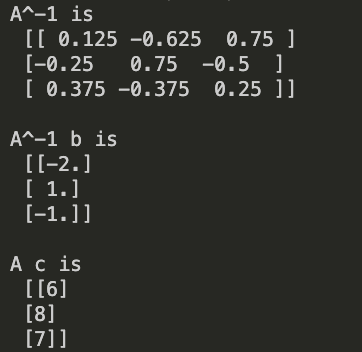
\includegraphics[width=8cm]{ps0_6_1}
  \centering
  \end{figure}

  \newpage
  \item 
  I chose $n=1000$. The resulting graph is
  \begin{figure}[h]
  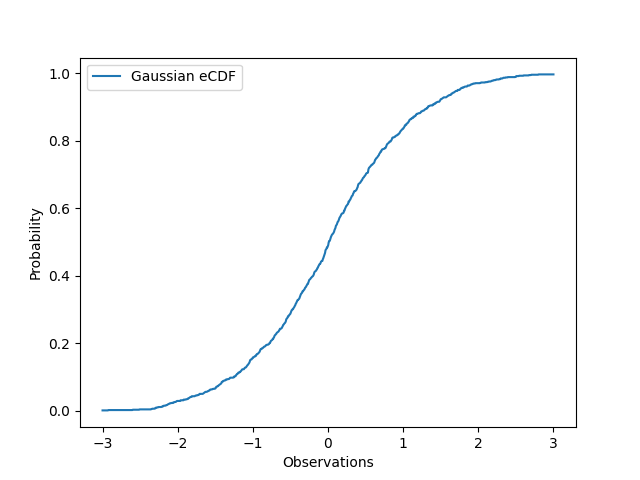
\includegraphics[width=15cm]{ps0_6_2_a}
  \centering
  \end{figure}

  \newpage
  \item 
  The resulting graph is
  \begin{figure}[h]
  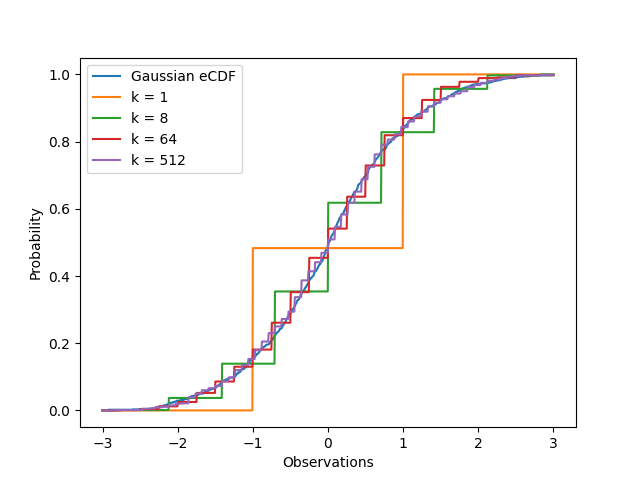
\includegraphics[width=15cm]{ps0_6_2_b}
  \centering
  \end{figure}
\end{enumerate}

\end{enumerate}





\end{document}
